\documentclass[twocolumn, 12pt]{article}

\usepackage[utf8]{inputenc}
\usepackage[english, spanish]{babel}
\usepackage{fullpage}
\usepackage{graphicx}
\usepackage{amsmath}
\usepackage{enumitem}
\usepackage{chngcntr}
\usepackage{setspace}
\usepackage{url}
\usepackage{csquotes}
\usepackage{float}
\usepackage{verbatim}
\usepackage{tabularx}
\usepackage{amsmath}
\usepackage{caption}
\usepackage{bm}
\usepackage{colortbl}
\usepackage{xcolor}

\usepackage{multirow}

% \usepackage{hyperref}

\definecolor{LigthGray}{rgb}{0.7098, 0.7294, 0.7215}
\definecolor{LigthGrayPlus}{rgb}{0.6862, 0.7254, 0.7294}
\definecolor{White}{rgb}{1, 1, 1}
\definecolor{Red}{rgb}{1, 0, 0}

\counterwithin{figure}{section}
\renewcommand{\thesection}{\arabic{section}}
\renewcommand{\thesubsection}{\thesection.\arabic{subsection}}
\renewcommand{\baselinestretch}{1.5}

\usepackage[style=numeric, maxnames=6, minnames=3, backend=biber, parentracker=true, sorting=none]{biblatex}
\DefineBibliographyStrings{english}{%chktex-file 1 chktex-file 6
      andothers = {\em et\addabbrvspace al\adddot}
}
\addbibresource{./Bibliography/bibliography.bib}

\usepackage{array}

\setlength{\parskip}{0pt}

\raggedbottom{}

\newcommand{\bolditalic}[1]{\textbf{\textit{#1}}}

\begin{document}

\begin{titlepage}
      \centering
      
\includegraphics[width=0.3\textwidth]{Images/logo_utb.png}\par\vspace{1cm}
      {\scshape\LARGE Universidad Tecnológica de Bolívar \par}
      \vspace{1cm}

      {\scshape\Large FÍSICA CALOR Y ONDAS \par}
      \vspace{.2cm}

      % chktex-file 8
      {\scshape\Large Grupo 1 \par}
      \vspace{1cm}
      % chktex-file 8
      \slshape {\Large \bfseries{}Informe de Laboratorio No. III\\}
      \slshape {\small \bfseries{}DIFRACCIÓN DE LA LUZ}
      \vspace{2cm}

      \slshape {\itshape{} Mauro González, T00067622 \\}
      \slshape {\itshape{} German De Armas Castaño, T00068765 \\}
      \slshape {\itshape{} Angel Vega Rodriguez, T00068186 \\}
      \slshape {\itshape{} Juan Jose Osorio Ariza, T00067316 \\}
      \slshape {\itshape{} Jorge Alberto Rueda Salgado, T00068722 \\}
      \vfill
      Revisado Por \\
      Duban Andres Paternina Verona\\
      {\large \today\par}
\end{titlepage}

% chktex-file 44
% chktex-file 24

% ! ----------------------------------------------------------------------|>
\section{Introducción}

La difracción de la luz es un fenómeno fascinante que nos
permite comprender cómo la luz se comporta cuando pasa a
través de obstáculos o se dispersa por rendijas estrechas.
Este fenómeno es esencial en la óptica y nos brinda
información valiosa sobre las propiedades de la luz. En
esta experiencia de laboratorio, exploraremos la difracción
de la luz utilizando una rejilla de difracción y un láser
de semiconductor. A través de este experimento, podremos
observar y analizar patrones de interferencia que se forman
cuando la luz se difracta en una rejilla.

% ! ----------------------------------------------------------------------|>
\section{Objetivos}

% + ----------------------------------------|>
\subsection{Objetivo general}

\begin{itemize}[label=$\triangleright$]
      \item El objetivo principal de esta experiencia de laboratorio es
            observar y comprender el fenómeno de difracción de la luz.
            A través de la utilización de una rejilla de difracción y
            un láser de semiconductor, buscaremos analizar y
            caracterizar los patrones de interferencia resultantes de
            la difracción de la luz. Además, se pretende determinar la
            longitud de onda de emisión del láser utilizando los
            patrones de difracción.
\end{itemize}

% + ----------------------------------------|>
\subsection{Objetivos específicos}

\begin{itemize}[label=$\triangleright$]
      \item Utilizar el patrón de difracción para determinar la
            longitud de onda de emisión del láser de semiconductor.

      \item Comparar los resultados experimentales obtenidos en el
            laboratorio con los valores teóricos esperados y verificar
            la precisión del fenómeno de difracción.

      \item Comprender el principio de Huygens y su relación con la
            difracción de la luz.

      \item Explorar la influencia del número de líneas por centímetro
            de la rejilla de difracción en la formación de los patrones
            de interferencia.
\end{itemize}

% ! ----------------------------------------------------------------------|>
\section{Marco Teórico}

% + -------------------------------------------------------------|>
\subsection{La luz~\cite{luz}}

es un espectro de onda electromagnética la cual es visible
por el ojo humano, la luz está compuesta por fotones, es
una forma de energía se desplaza en línea recta a una
velocidad constante como emisión ondulatoria de fotones,
tiene longitudes de ondas las cuales son responsables del
color del espectro visible. [1]

% + -------------------------------------------------------------|>
\subsection{Luz monocromática~\cite{Tamiko_2023}}

esta se caracteriza por ser de un único color, está
compuesta por una única longitud de onda, esta puede
experimentar diversos fenómenos como la difracción,
reflexión y la refracción, en esta experiencia nos
enfocaremos en la difracción de un láser
(monocromático).[2]

% + -------------------------------------------------------------|>
\subsection{Principio de Huygens}

El principio de Huygens nos permite explicar cómo una onda
luminosa se propaga a través del espacio y cómo se comporta
cuando encuentra obstáculos o pasa por aperturas. En este
principio se enuncia que: “Cada punto en un frente de onda
de una onda luminosa es una fuente secundaria de ondas
esféricas. La nueva onda se forma a partir de la
superposición de estas ondas esféricas.”

\begin{quotation}
      ``Cada punto en un frente de onda de una onda luminosa
      es una fuente secundaria de ondas esféricas. La nueva
      onda se forma a partir de la superposición de estas
      ondas esféricas''.
\end{quotation}

\begin{figure}[H]
      \begin{center}
            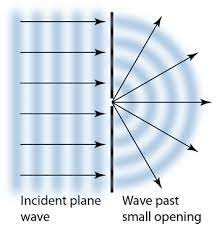
\includegraphics[width=.9\linewidth]{./Images/5.jpg}
      \end{center}
      \caption{}
\end{figure}

% + -------------------------------------------------------------|>
\subsection{Difracción}

La difracción es un fenómeno que ocurre cuando una onda (en
este caso la luz), pasa por una abertura o un obstáculo y
se curva o se dispersa alrededor de ese obstáculo. Este
fenómeno es una consecuencia de la naturaleza ondulatoria
de las ondas y puede observarse en diversas situaciones. En
el contexto de la luz, la difracción puede ocurrir cuando
la luz pasa a través de una rendija estrecha, una apertura
circular, una red de difracción u otros tipos de obstáculos
o estructuras que interrumpen su trayectoria.

\begin{figure}[H]
      \begin{center}
            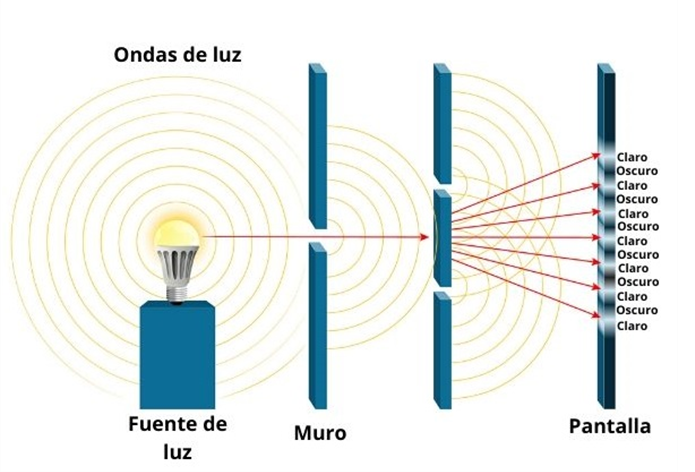
\includegraphics[width=.9\linewidth]{./Images/6.png}
      \end{center}
      \caption{}
\end{figure}

% + -------------------------------------------------------------|>
\subsection{Difracción de Fraunhofer}

A una longitud de onda dada, la teoría de Fraunhofer
predice la ubicación angular de los máximos y mínimos de la
dispersión en función del tamaño de un
objeto.~\cite{fraunhofer}Para obtener un patrón de
difracción de Fraunhofer, se requiere que se cumplan una
serie de condiciones específicas relacionadas con la
geometría y la distancia entre la fuente de luz, la
abertura u obstáculo, y la pantalla o superficie receptora
donde se observa el patrón de difracción.

\subsubsection*{Difracción de Fraunhofer \hfill{} \break{} para una abertura rectangular}

\begin{equation*}
      \sen (\theta) = n(\frac{\lambda}{b})
\end{equation*}

% + -------------------------------------------------------------|>
\subsection*{Formulas a utilizar}

{\Large
      \begin{equation}
            \lambda_{n} = \frac{d \cdot \sen ( \tan^{-1} (\frac{X_{n}}{D}))}{n}
            \label{eq:lambda-n}
      \end{equation}
}

{\Large
      \begin{equation}
            \mathcal{G}_x = \frac{\lambda D}{x}
            \label{eq:grosor-cabello}
      \end{equation}
}

{\Large
      \begin{equation}
            x_{n} = D \frac{n \lambda}{G_{c}}
            \label{eq:x_n}
      \end{equation}
}

% ! ----------------------------------------------------------------------|>
\section{Montaje Experimental}

\begin{figure}[H]
      \begin{center}
            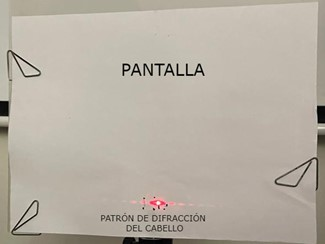
\includegraphics[width=.9\linewidth]{./Images/1.jpg}
            \caption{}
      \end{center}
\end{figure}

\vspace{-.5cm}

\begin{figure}[H]
      \begin{center}
            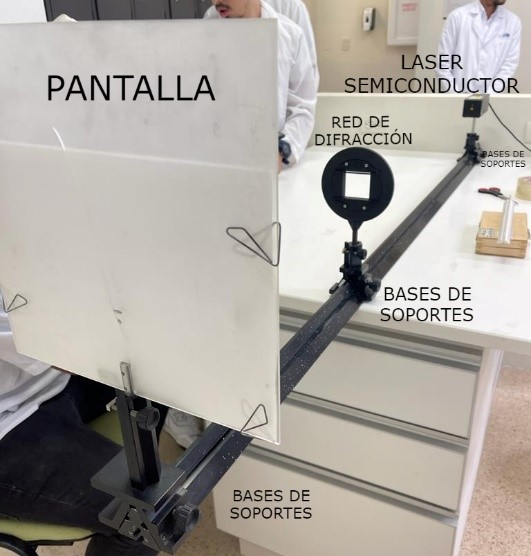
\includegraphics[width=.9\linewidth]{./Images/2.jpg}
            \caption{}
      \end{center}
\end{figure}

\vspace{-.5cm}

\begin{figure}[H]
      \begin{center}
            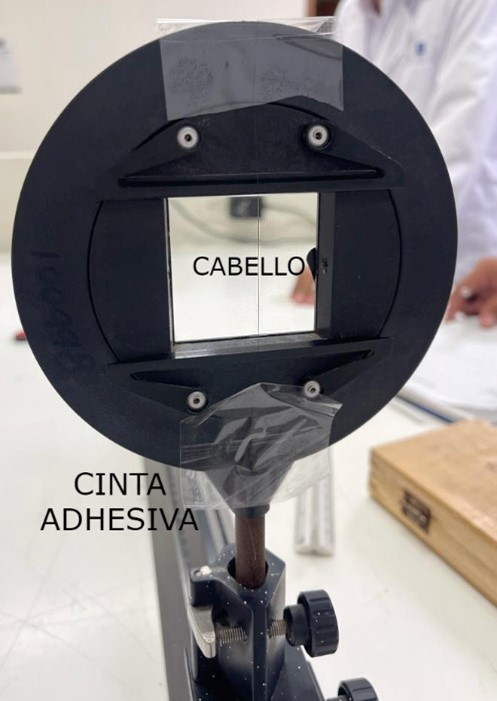
\includegraphics[width=.9\linewidth]{./Images/3.jpg}
            \caption{}
      \end{center}
\end{figure}

\vspace{-.5cm}

\begin{figure}[H]
      \begin{center}
            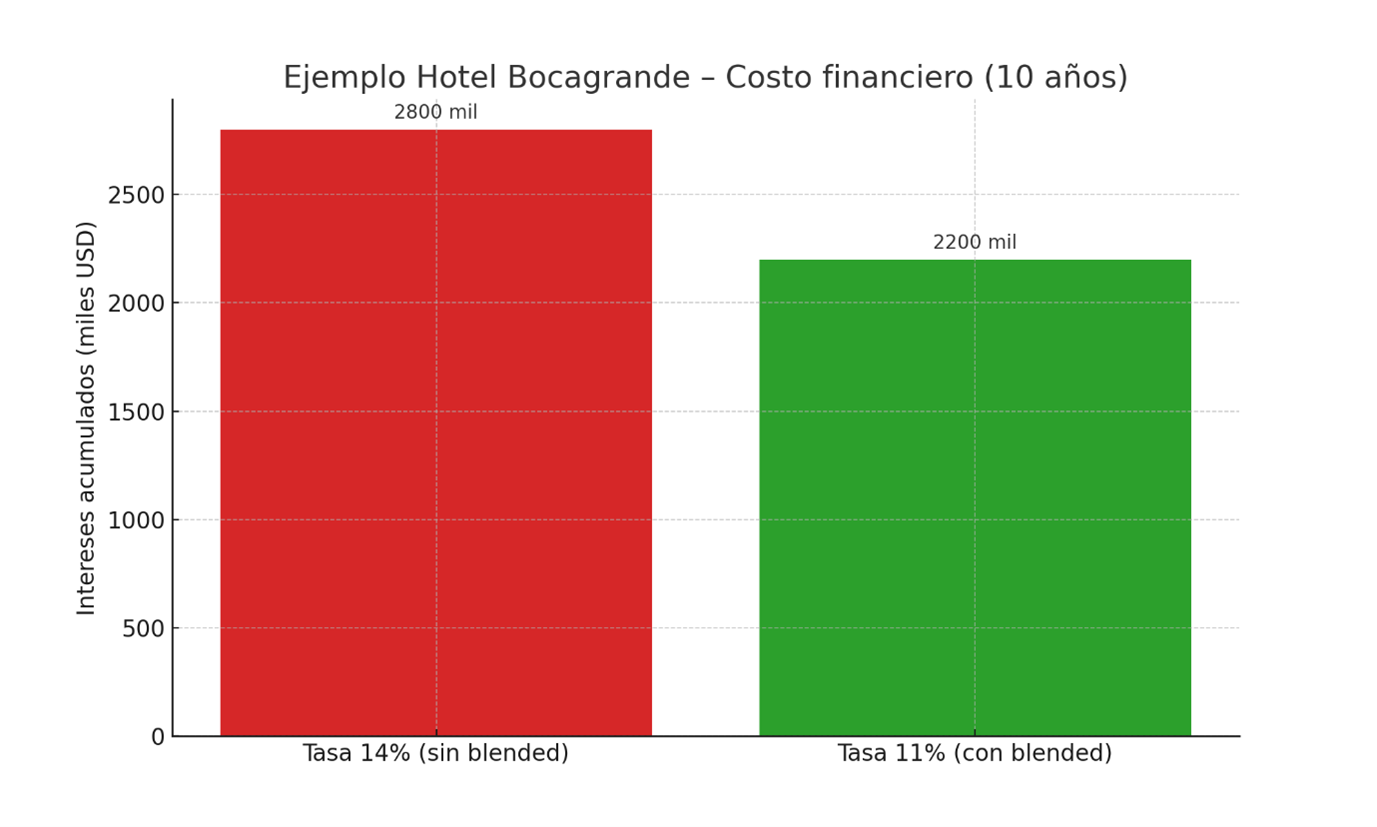
\includegraphics[width=.9\linewidth]{./Images/4.png}
            \caption{}
      \end{center}
\end{figure}

Equipo usado:

\begin{itemize}[label=$\triangleright$]
      \item 1 Laser semiconductor.
      \item 1 Red de difracción.
      \item 3 Bases de soporte.
      \item 1 Pantalla.
      \item 1 Calibrador micrométrico.
\end{itemize}

En esta experiencia realizamos dos experimentos; la
difracción de la luz debido a una rejilla y la difracción
de la luz debido a un cabello con ayuda del montaje
expuesto anteriormente, en el que luego de encender el
laser y estar la rejilla de difracción o en su defecto el
cabello, medir cada uno de los máximos obtenidos x (m) en
el patrón de difracción reflejado en la pantalla, variando
la distancia de la rejilla a esta, para posteriormente con
los datos obtenidos y debidamente registrados calcular el
valor del ángulo $\theta$ y la longitud de onda $\lambda$.

% ! ----------------------------------------------------------------------|>
\section{Datos Experimentales}

\begin{table}[H]
      \begin{center}
            \begin{tabularx}{\linewidth}{|>{\centering\arraybackslash}X|>{\centering\arraybackslash}X|>{\centering\arraybackslash}X|}
                  \multicolumn{3}{c}{$D_{1} = 0,7111$ \bolditalic{(m)}}                                                                                \\\hline
                  \multirow{3}{*}{\textbf{n}} & \multirow{3}{*}{$x$ \bolditalic{(m)}} & {\Large $\lambda_{n}$} \bolditalic{(mm)} \break{} Experimental \\\hline
                  1                           & $4,50 \cdot 10^{-02}$                 & $6,32 \cdot 10^{-04}$                                          \\\hline

                  2                           & $9,00 \cdot 10^{-02}$                 & $6,29 \cdot 10^{-04}$                                          \\\hline

                  3                           & $1,37 \cdot 10^{-01}$                 & $6,34 \cdot 10^{-04}$                                          \\\hline

            \end{tabularx}

            \vspace{-.02cm}

            \begin{tabularx}{\linewidth}{|>{\centering\arraybackslash}X|>{\centering\arraybackslash}X|}
                  {\large $\lambda_{Promedio}$} \bolditalic{(mm)} & $6,32 \cdot 10^{-4}$ \\\hline
            \end{tabularx}
      \end{center}
      \caption{}
      \label{tab:d1}
\end{table}

\begin{table}[H]
      \begin{center}
            \begin{tabularx}{\linewidth}{|>{\centering\arraybackslash}X|>{\centering\arraybackslash}X|>{\centering\arraybackslash}X|}
                  \multicolumn{3}{c}{$D_{2} = 0,4500$ \bolditalic{(m)}}                                                                                \\\hline
                  \multirow{3}{*}{\textbf{n}} & \multirow{3}{*}{$x$ \bolditalic{(m)}} & {\Large $\lambda_{n}$} \bolditalic{(mm)} \break{} Experimental \\\hline
                  1                           & $2,80 \cdot 10^{-02}$                 & $6,21 \cdot 10^{-04}$                                          \\\hline

                  2                           & $5,70 \cdot 10^{-02}$                 & $6,30 \cdot 10^{-04}$                                          \\\hline

                  3                           & $8,70 \cdot 10^{-02}$                 & $6,36 \cdot 10^{-04}$                                          \\\hline

            \end{tabularx}

            \vspace{-.02cm}

            \begin{tabularx}{\linewidth}{|>{\centering\arraybackslash}X|>{\centering\arraybackslash}X|}
                  {\large $\lambda_{Promedio}$} \bolditalic{(mm)} & $6,29 \cdot 10^{-4}$ \\\hline
            \end{tabularx}
      \end{center}
      \caption{}
      \label{tab:d2}
\end{table}

\begin{table}[H]
      \begin{center}
            \begin{tabularx}{\linewidth}{|>{\centering\arraybackslash}X|>{\centering\arraybackslash}X|}
                  \multicolumn{2}{c}{Datos (Grosor de un cabello)}                                 \\\hline
                  \textbf{D} \bolditalic{(m)}                                            & $1,48$  \\\hline
                  $\lambda$ \bolditalic{(nm)}~\footnote{Proporcionado por el fabricante} & $632,8$ \\\hline
                  $x_{Experimental}$ \bolditalic{(cm)}                                   & $0,8$   \\\hline
            \end{tabularx}

            \vspace{-.02cm}

            \begin{tabularx}{\linewidth}{|>{\centering\arraybackslash}X|}
                  Grosor experimental \bolditalic{(mm)} \\\hline
                  $0,0750$                              \\\hline
            \end{tabularx}
      \end{center}
      \caption{}
      \label{tab:g}
\end{table}

% ! ----------------------------------------------------------------------|>
\section{Análisis de datos}

% + -------------------------------------------------------------|>
\subsection{Análisis}

% * ------------------------------------------------------|>
\subsubsection{}

\begin{table}[H]
      \begin{center}
            \begin{tabularx}{\linewidth}{|>{\centering\arraybackslash}X|>{\centering\arraybackslash}X|}
                  \hline
                  {\large $\lambda_{Teorico}$} \bolditalic{(nm)} & $632,8$ \\\hline
            \end{tabularx}
      \end{center}
\end{table}

\vspace{-.5cm}

\begin{table}[H]
      \begin{center}
            \begin{tabularx}{\linewidth}{|>{\centering\arraybackslash}X|>{\centering\arraybackslash}X|}
                  \multicolumn{2}{c}{$D_{1}$}          \\\hline
                  \textbf{n} & Error \bolditalic{(\%)} \\\hline
                  1          & $0,20$                  \\\hline

                  2          & $0,59$                  \\\hline

                  3          & $0,19$                  \\\hline

            \end{tabularx}
      \end{center}
      \caption{}
\end{table}

\begin{table}[H]
      \begin{center}
            \begin{tabularx}{\linewidth}{|>{\centering\arraybackslash}X|>{\centering\arraybackslash}X|}
                  \multicolumn{2}{c}{$D_{1}$}          \\\hline
                  \textbf{n} & Error \bolditalic{(\%)} \\\hline
                  1          & $1,86$                  \\\hline

                  2          & $0,51$                  \\\hline

                  3          & $0,53$                  \\\hline

            \end{tabularx}
      \end{center}
      \caption{}
\end{table}

% * ------------------------------------------------------|>
\subsubsection{}

Usando los datos de la tabla~(\ref{tab:g}) y la
formula~(\ref{eq:grosor-cabello}) y~(\ref{eq:x_n}),

\begin{equation*}
      \begin{gathered}
            x_{n} = 1480 mm \cdot \frac{6,328 \times 10^{-4}}{0,0750} \\
            x_{n} = 12,48 mm \approx 12 mm
      \end{gathered}
\end{equation*}

\noindent\makebox[\linewidth]{\rule{\linewidth}{0.4pt}}

\begin{equation*}
      \begin{gathered}
            G_{c} = 1480 mm \cdot \frac{6,328 \times 10^{-4}}{12mm} \\
            G_{c} = 0,0780 mm
      \end{gathered}
\end{equation*}

\begin{table}[H]
      \begin{center}
            \begin{tabularx}{\linewidth}{|>{\centering\arraybackslash}X|>{\centering\arraybackslash}X|}
                  \hline
                  Error \bolditalic{(\%)} & $3,85$ \\\hline
            \end{tabularx}
      \end{center}
\end{table}

% * ------------------------------------------------------|>
\subsubsection{}

Para que la luz láser experimente una difracción apreciable
al pasar a través de una abertura u obstáculo, las
dimensiones de la abertura u obstáculo deben ser del mismo
orden de magnitud o de tamaño similar a la longitud de onda
de la luz láser que se está utilizando.

Esto significa que las dimensiones de la abertura u
obstáculo deben ser comparables a la longitud de onda de la
luz láser si el tamaño de la abertura u obstáculo es del
mismo orden de magnitud que la mitad de la longitud de onda
$(\lambda/2)$ o más pequeño, se producirá una difracción
apreciable.

% * ------------------------------------------------------|>
\subsubsection{}

El patrón de difracción generado por una ranura y el de un
cabello con las mismas dimensiones de la ranura pueden ser
diferentes debido a las características intrínsecas de los
dos objetos y la naturaleza de la difracción en cada caso.

A pesar de que una ranura y un cabello puedan compartir
dimensiones físicas similares, las diferencias en su forma,
estructura y superficie pueden resultar en patrones de
difracción distintos cuando se exponen a la luz láser. La
manera en que la luz se comporta al interactuar con estos
objetos está influenciada por sus características
particulares, lo que puede dar como resultado la generación
de patrones de difracción diversos.

% * ------------------------------------------------------|>
\subsubsection{}

El fenómeno de difracción no es exclusivo de las ondas,
pero es más comúnmente asociado con el comportamiento de
las ondas, como las ondas de luz, sonido o agua. Sin
embargo, es importante destacar que la difracción también
puede ocurrir con partículas, como electrones y átomos, por
lo tanto, aunque la difracción es más comúnmente asociada
con ondas, también puede manifestarse en el comportamiento
de partículas, lo que demuestra sus usos en diferentes
contextos físicos.

% * ------------------------------------------------------|>
\subsubsection{}

Sí, la luz se puede estudiar y entender como una onda, y
esta perspectiva ha sido fundamental en la física y la
óptica, la descripción de la luz como una onda ha
demostrado ser exitosa en la explicación de una amplia gama
de fenómenos observados, esta perspectiva se respalda
mediante numerosos experimentos que han confirmado que la
luz está compuesta por ondas y que su comportamiento puede
describirse mediante relaciones matemáticas. Además, la luz
exhibe fenómenos notables de interferencia y difracción,
que son características típicas de los comportamientos
ondulatorios.

% ! ----------------------------------------------------------------------|>
\section{Conclusiones}

En este experimento de laboratorio, hemos explorado el
fenómeno de la difracción de la luz utilizando un láser que
pasa a través de una abertura u obstáculo. Nuestros
resultados han demostrado claramente que la difracción es
un fenómeno fundamental que afecta la propagación de la luz
cuando esta interactúa con obstáculos o aperturas en su
camino. Hemos observado que cuando la luz láser pasa a
través de una ranura de dimensiones físicas similares a la
longitud de onda de la luz, se produce una difracción
significativa.

Esto se manifiesta como patrones de franjas brillantes y
oscuras en la pantalla de detección, conocidos como
patrones de difracción. Estos patrones de difracción son
una consecuencia directa del principio de Huygens-Fresnel,
que postula que cada punto en una onda incidente puede ser
considerado como una fuente de ondas secundarias que se
suman para formar el patrón de difracción. Cuando
comparamos los resultados obtenidos con una ranura y un
cabello de dimensiones físicas similares, encontramos una
diferencia notable en los patrones de difracción. En el
caso de la ranura, se obtiene un patrón de difracción
característico con franjas de intensidad alternante. Sin
embargo, cuando se utiliza un cabello, el patrón de
difracción es menos definido y más complejo.Esto se debe a
que la forma y las irregularidades en la superficie del
cabello introducen múltiples fuentes de difracción, lo que
resulta en un patrón de difracción más difuso y menos
ordenado.

ste experimento ha destacado la importancia de la
difracción de la luz en la interacción de la luz con
obstáculos o aberturas. Además, hemos observado que la
difracción es más pronunciada cuando se utiliza una ranura
en comparación con un cabello de dimensiones físicas
similares debido a las diferencias en la forma y las
irregularidades de la superficie.

\printbibliography

\end{document}